% Options for packages loaded elsewhere
\PassOptionsToPackage{unicode}{hyperref}
\PassOptionsToPackage{hyphens}{url}
\documentclass[
  ignorenonframetext,
]{beamer}
\newif\ifbibliography
\usepackage{pgfpages}
\setbeamertemplate{caption}[numbered]
\setbeamertemplate{caption label separator}{: }
\setbeamercolor{caption name}{fg=normal text.fg}
\beamertemplatenavigationsymbolsempty
% remove section numbering
\setbeamertemplate{part page}{
  \centering
  \begin{beamercolorbox}[sep=16pt,center]{part title}
    \usebeamerfont{part title}\insertpart\par
  \end{beamercolorbox}
}
\setbeamertemplate{section page}{
  \centering
  \begin{beamercolorbox}[sep=12pt,center]{section title}
    \usebeamerfont{section title}\insertsection\par
  \end{beamercolorbox}
}
\setbeamertemplate{subsection page}{
  \centering
  \begin{beamercolorbox}[sep=8pt,center]{subsection title}
    \usebeamerfont{subsection title}\insertsubsection\par
  \end{beamercolorbox}
}
% Prevent slide breaks in the middle of a paragraph
\widowpenalties 1 10000
\raggedbottom
\AtBeginPart{
  \frame{\partpage}
}
\AtBeginSection{
  \ifbibliography
  \else
    \frame{\sectionpage}
  \fi
}
\AtBeginSubsection{
  \frame{\subsectionpage}
}
\usepackage{iftex}
\ifPDFTeX
  \usepackage[T1]{fontenc}
  \usepackage[utf8]{inputenc}
  \usepackage{textcomp} % provide euro and other symbols
\else % if luatex or xetex
  \usepackage{unicode-math} % this also loads fontspec
  \defaultfontfeatures{Scale=MatchLowercase}
  \defaultfontfeatures[\rmfamily]{Ligatures=TeX,Scale=1}
\fi
\usepackage{lmodern}
\ifPDFTeX\else
  % xetex/luatex font selection
\fi
% Use upquote if available, for straight quotes in verbatim environments
\IfFileExists{upquote.sty}{\usepackage{upquote}}{}
\IfFileExists{microtype.sty}{% use microtype if available
  \usepackage[]{microtype}
  \UseMicrotypeSet[protrusion]{basicmath} % disable protrusion for tt fonts
}{}
\makeatletter
\@ifundefined{KOMAClassName}{% if non-KOMA class
  \IfFileExists{parskip.sty}{%
    \usepackage{parskip}
  }{% else
    \setlength{\parindent}{0pt}
    \setlength{\parskip}{6pt plus 2pt minus 1pt}}
}{% if KOMA class
  \KOMAoptions{parskip=half}}
\makeatother
\usepackage{graphicx}
\makeatletter
\newsavebox\pandoc@box
\newcommand*\pandocbounded[1]{% scales image to fit in text height/width
  \sbox\pandoc@box{#1}%
  \Gscale@div\@tempa{\textheight}{\dimexpr\ht\pandoc@box+\dp\pandoc@box\relax}%
  \Gscale@div\@tempb{\linewidth}{\wd\pandoc@box}%
  \ifdim\@tempb\p@<\@tempa\p@\let\@tempa\@tempb\fi% select the smaller of both
  \ifdim\@tempa\p@<\p@\scalebox{\@tempa}{\usebox\pandoc@box}%
  \else\usebox{\pandoc@box}%
  \fi%
}
% Set default figure placement to htbp
\def\fps@figure{htbp}
\makeatother
% definitions for citeproc citations
\NewDocumentCommand\citeproctext{}{}
\NewDocumentCommand\citeproc{mm}{%
  \begingroup\def\citeproctext{#2}\cite{#1}\endgroup}
\makeatletter
 % allow citations to break across lines
 \let\@cite@ofmt\@firstofone
 % avoid brackets around text for \cite:
 \def\@biblabel#1{}
 \def\@cite#1#2{{#1\if@tempswa , #2\fi}}
\makeatother
\newlength{\cslhangindent}
\setlength{\cslhangindent}{1.5em}
\newlength{\csllabelwidth}
\setlength{\csllabelwidth}{3em}
\newenvironment{CSLReferences}[2] % #1 hanging-indent, #2 entry-spacing
 {\begin{list}{}{%
  \setlength{\itemindent}{0pt}
  \setlength{\leftmargin}{0pt}
  \setlength{\parsep}{0pt}
  % turn on hanging indent if param 1 is 1
  \ifodd #1
   \setlength{\leftmargin}{\cslhangindent}
   \setlength{\itemindent}{-1\cslhangindent}
  \fi
  % set entry spacing
  \setlength{\itemsep}{#2\baselineskip}}}
 {\end{list}}
\usepackage{calc}
\newcommand{\CSLBlock}[1]{\hfill\break\parbox[t]{\linewidth}{\strut\ignorespaces#1\strut}}
\newcommand{\CSLLeftMargin}[1]{\parbox[t]{\csllabelwidth}{\strut#1\strut}}
\newcommand{\CSLRightInline}[1]{\parbox[t]{\linewidth - \csllabelwidth}{\strut#1\strut}}
\newcommand{\CSLIndent}[1]{\hspace{\cslhangindent}#1}
\setlength{\emergencystretch}{3em} % prevent overfull lines
\providecommand{\tightlist}{%
  \setlength{\itemsep}{0pt}\setlength{\parskip}{0pt}}
\usepackage{bookmark}
\IfFileExists{xurl.sty}{\usepackage{xurl}}{} % add URL line breaks if available
\urlstyle{same}
\hypersetup{
  pdftitle={Homologias{,} Caracteres e Mensurações},
  pdfauthor={Guilherme Garcia; Diogo Melo},
  hidelinks,
  pdfcreator={LaTeX via pandoc}}

\title{\texorpdfstring{Homologias, Caracteres e
Mensurações}{Homologias{,} Caracteres e Mensurações}}
\subtitle{\texorpdfstring{Modularidade: conectando padrões e processos
em evolução
multivariada}{Modularidade: conectando padrões e processos em evolução multivariada}}
\author{\texorpdfstring{Guilherme Garcia \and Diogo
Melo}{Guilherme Garcia; Diogo Melo}}
\date{\href{mailto:damelo@ib.usp.br}{\nolinkurl{damelo@ib.usp.br}}}
\logo{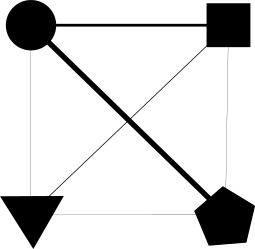
\includegraphics{../../logo.png}}

\begin{document}
\frame{\titlepage}

\begin{frame}{Objetivos}
\protect\phantomsection\label{objetivos}
\begin{itemize}[<+->]
\tightlist
\item
  Relacionar o contexto teórico de um fenômeno de interesse às formas de
  mensurar seus efeitos
\end{itemize}

\begin{itemize}[<+->]
\tightlist
\item
  Elaborar esta relação a respeito de sistemas morfológicos, seu
  desenvolvimento e função
\end{itemize}

\begin{block}{Homologias}
\protect\phantomsection\label{homologias}
\begin{itemize}
\item
  Relações de equivalência entre atributos em espécies distintas

  \begin{itemize}[<+->]
  \tightlist
  \item
    Revelam origens evolutivas em comum
  \end{itemize}

  \begin{itemize}[<+->]
  \tightlist
  \item
    Vias de desenvolvimento compartilhadas
  \end{itemize}

  \begin{itemize}[<+->]
  \tightlist
  \item
    Relação global entre atributos
  \end{itemize}
\end{itemize}
\end{block}

\begin{block}{Um exemplo mais extremo}
\protect\phantomsection\label{um-exemplo-mais-extremo}
\begin{figure}
\centering
\pandocbounded{
\includegraphics[keepaspectratio,alt={(Tulenko et al. 2016)}]{index_files/figures/forelimb_phylo.png}}
\caption{(Tulenko et al. 2016)}
\end{figure}
\end{block}

\begin{block}{}
\protect\phantomsection\label{section}
\begin{itemize}[<+->]
\tightlist
\item
  Desenvolvimento dos elementos ósseos determinado pela expressão dos
  mesmos \emph{loci} nas três linhagens
\end{itemize}

~

\begin{itemize}[<+->]
\tightlist
\item
  Elementos ósseos adicionais nas linhagens derivadas regulados pelos
  mesmos \emph{loci} em uma fase posterior
\end{itemize}

\begin{figure}
\centering
\pandocbounded{
\includegraphics[keepaspectratio,alt={(Yano and Tamura 2013)}]{index_files/figures/hox_homology.png}}
\caption{(Yano and Tamura 2013)}
\end{figure}
\end{block}

\begin{block}{Homologias e Mapas Genótipo-Fenótipo}
\protect\phantomsection\label{homologias-e-mapas-genuxf3tipo-fenuxf3tipo}
\pandocbounded{
\includegraphics[keepaspectratio]{index_files/figures/gpmap_homology_1.png}}
\end{block}

\begin{block}{Homologias e Mapas Genótipo-Fenótipo}
\protect\phantomsection\label{homologias-e-mapas-genuxf3tipo-fenuxf3tipo-1}
\pandocbounded{
\includegraphics[keepaspectratio]{index_files/figures/gpmap_homology_2.png}}
\end{block}

\begin{block}{Como reconhecer homologias?}
\protect\phantomsection\label{como-reconhecer-homologias}
\end{block}

\begin{block}{Caráter}
\protect\phantomsection\label{caruxe1ter}
Conjunto de atributos \emph{mutuamente exclusivos} identificados em um
conjunto de organismos

\begin{itemize}[<+->]
\tightlist
\item
  \emph{Mutuamente exclusivos}: a cada organismo atribui-se apenas um
  estado do caráter
\end{itemize}
\end{block}

\begin{block}{Exemplo: Coloração}
\protect\phantomsection\label{exemplo-colorauxe7uxe3o}
\pandocbounded{
\includegraphics[keepaspectratio]{index_files/figures/lizard_set_0.png}}
\end{block}

\begin{block}{Exemplo: Coloração}
\protect\phantomsection\label{exemplo-colorauxe7uxe3o-1}
\pandocbounded{
\includegraphics[keepaspectratio]{index_files/figures/lizard_set_1.png}}
\end{block}

\begin{block}{Exemplo: Coloração}
\protect\phantomsection\label{exemplo-colorauxe7uxe3o-2}
\pandocbounded{
\includegraphics[keepaspectratio]{index_files/figures/lizard_set_2.png}}
\end{block}

\begin{block}{Exemplo: Coloração}
\protect\phantomsection\label{exemplo-colorauxe7uxe3o-3}
\pandocbounded{
\includegraphics[keepaspectratio]{index_files/figures/lizard_set_3.png}}
\end{block}

\begin{block}{Em princípio\ldots{}}
\protect\phantomsection\label{em-princuxedpio}
\begin{itemize}[<+->]
\tightlist
\item
  Homologias não aparecem nesta definição de caráter
\end{itemize}

\begin{itemize}[<+->]
\tightlist
\item
  Caracteres são divisões arbitrárias que somos capazes de reconhecer em
  organismos ou suas partes
\end{itemize}

\begin{itemize}[<+->]
\tightlist
\item
  O uso de um conjunto particular de caracteres se justifica com base no
  contexto teórico de referência
\end{itemize}
\end{block}

\begin{block}{}
\protect\phantomsection\label{section-1}
\begin{figure}
\centering
\pandocbounded{
\includegraphics[keepaspectratio,alt={(Levins and Lewontin 1985; Houle et al. 2011)}]{index_files/figures/dial_1.png}}
\caption{(Levins and Lewontin 1985; Houle et al. 2011)}
\end{figure}
\end{block}

\begin{block}{}
\protect\phantomsection\label{section-2}
\begin{figure}
\centering
\pandocbounded{
\includegraphics[keepaspectratio,alt={(Levins and Lewontin 1985; Houle et al. 2011)}]{index_files/figures/dial_2.png}}
\caption{(Levins and Lewontin 1985; Houle et al. 2011)}
\end{figure}
\end{block}

\begin{block}{}
\protect\phantomsection\label{section-3}
\begin{figure}
\centering
\pandocbounded{
\includegraphics[keepaspectratio,alt={(Levins and Lewontin 1985; Houle et al. 2011)}]{index_files/figures/dial_3.png}}
\caption{(Levins and Lewontin 1985; Houle et al. 2011)}
\end{figure}
\end{block}

\begin{block}{}
\protect\phantomsection\label{section-4}
\begin{figure}
\centering
\pandocbounded{
\includegraphics[keepaspectratio,alt={(Levins and Lewontin 1985; Houle et al. 2011)}]{index_files/figures/dial_4.png}}
\caption{(Levins and Lewontin 1985; Houle et al. 2011)}
\end{figure}
\end{block}

\begin{block}{Mensuração}
\protect\phantomsection\label{mensurauxe7uxe3o}
\begin{itemize}[<+->]
\tightlist
\item
  \emph{Estrutura de relações empíricas}: objetos reais, seus atributos
  e o conjunto de operações sobre eles
\end{itemize}

\begin{itemize}[<+->]
\tightlist
\item
  \emph{Estrutura de relações numéricas}: valores/estados dos atributos
  e o conjunto de operações válidas entre estes valores
\end{itemize}

\begin{itemize}[<+->]
\tightlist
\item
  \textbf{Mensuração}: Relação de equivalência entre estas estruturas
\end{itemize}
\end{block}

\begin{block}{}
\protect\phantomsection\label{section-5}
\begin{figure}
\centering
\pandocbounded{
\includegraphics[keepaspectratio,alt={(Levins and Lewontin 1985; Houle et al. 2011)}]{index_files/figures/dial_4.png}}
\caption{(Levins and Lewontin 1985; Houle et al. 2011)}
\end{figure}
\end{block}

\begin{block}{}
\protect\phantomsection\label{section-6}
\begin{figure}
\centering
\pandocbounded{
\includegraphics[keepaspectratio,alt={(Levins and Lewontin 1985; Houle et al. 2011)}]{index_files/figures/dial_5.png}}
\caption{(Levins and Lewontin 1985; Houle et al. 2011)}
\end{figure}
\end{block}

\begin{block}{Temperatura}
\protect\phantomsection\label{temperatura}
\pandocbounded{
\includegraphics[keepaspectratio]{index_files/figures/temp_1.png}}
\end{block}

\begin{block}{Temperatura}
\protect\phantomsection\label{temperatura-1}
\pandocbounded{
\includegraphics[keepaspectratio]{index_files/figures/temp_2.png}}
\end{block}

\begin{block}{Temperatura}
\protect\phantomsection\label{temperatura-2}
\pandocbounded{
\includegraphics[keepaspectratio]{index_files/figures/temp_3.png}}
\end{block}

\begin{block}{Temperatura}
\protect\phantomsection\label{temperatura-3}
\pandocbounded{
\includegraphics[keepaspectratio]{index_files/figures/temp_4.png}}
\end{block}

\begin{block}{Temperatura}
\protect\phantomsection\label{temperatura-4}
\pandocbounded{
\includegraphics[keepaspectratio]{index_files/figures/temp_5.png}}
\end{block}

\begin{block}{Temperatura}
\protect\phantomsection\label{temperatura-5}
\pandocbounded{
\includegraphics[keepaspectratio]{index_files/figures/temp_6.png}}
\end{block}

\begin{block}{Temperatura}
\protect\phantomsection\label{temperatura-6}
\pandocbounded{
\includegraphics[keepaspectratio]{index_files/figures/temp_7.png}}
\end{block}

\begin{block}{}
\protect\phantomsection\label{section-7}
\begin{figure}
\centering
\pandocbounded{
\includegraphics[keepaspectratio,alt={(Houle et al. 2011)}]{index_files/figures/theory_to_measurement.png}}
\caption{(Houle et al. 2011)}
\end{figure}
\end{block}

\begin{block}{Tamanho e Peso}
\protect\phantomsection\label{tamanho-e-peso}
\pandocbounded{
\includegraphics[keepaspectratio]{index_files/figures/balance.png}}

\begin{itemize}[<+->]
\tightlist
\item
  Comparação entre objetos permite estrutura de produto nas relações
  numéricas
\end{itemize}

\begin{itemize}[<+->]
\tightlist
\item
  Passível de transformação para escala log
\end{itemize}
\end{block}

\begin{block}{Medidas de referência}
\protect\phantomsection\label{medidas-de-referuxeancia}
\end{block}

\begin{block}{Medidas de referência}
\protect\phantomsection\label{medidas-de-referuxeancia-1}
\end{block}

\begin{block}{Medidas de referência}
\protect\phantomsection\label{medidas-de-referuxeancia-2}
\end{block}

\begin{block}{}
\protect\phantomsection\label{section-8}
\begin{figure}
\centering
\pandocbounded{
\includegraphics[keepaspectratio,alt={(Houle et al. 2011)}]{index_files/figures/theory_to_measurement.png}}
\caption{(Houle et al. 2011)}
\end{figure}
\end{block}

\begin{block}{Medidas Pragmáticas}
\protect\phantomsection\label{medidas-pragmuxe1ticas}
\begin{itemize}
\tightlist
\item
  Como mensurar atratividade?
\end{itemize}

\begin{itemize}
\tightlist
\item
  Poderíamos fazer um experimento:
\end{itemize}

\pandocbounded{
\includegraphics[keepaspectratio]{index_files/figures/fishtank_1.png}}
\end{block}

\begin{block}{Medidas Pragmáticas}
\protect\phantomsection\label{medidas-pragmuxe1ticas-1}
\begin{itemize}
\item
  Como mensurar atratividade?
\item
  Poderíamos fazer um experimento:
\end{itemize}

\pandocbounded{
\includegraphics[keepaspectratio]{index_files/figures/fishtank_2.png}}
\end{block}

\begin{block}{Medidas Pragmáticas}
\protect\phantomsection\label{medidas-pragmuxe1ticas-2}
\begin{itemize}[<+->]
\tightlist
\item
  Algumas mensurações apenas aproximam o fenômeno de interesse
\end{itemize}

\begin{itemize}[<+->]
\tightlist
\item
  Aptidão, este atributo elusivo\ldots{}
\end{itemize}

\begin{itemize}[<+->]
\tightlist
\item
  Nunca se esqueça da distinção entre o fenômeno de interesse e a forma
  que você usa para representá-lo
\end{itemize}

\begin{itemize}[<+->]
\tightlist
\item
  Variável teórica -\textgreater{} Variável operacional
\end{itemize}
\end{block}

\begin{block}{Porque medir caracteres homólogos?}
\protect\phantomsection\label{porque-medir-caracteres-homuxf3logos}
\pandocbounded{
\includegraphics[keepaspectratio]{index_files/figures/gpmap_homology_2.png}}
\end{block}

\begin{block}{Quando não medir caracteres homólogos?}
\protect\phantomsection\label{quando-nuxe3o-medir-caracteres-homuxf3logos}
\pandocbounded{
\includegraphics[keepaspectratio]{index_files/figures/forelimb_phylo.png}}
\end{block}

\begin{block}{Quando não medir caracteres homólogos?}
\protect\phantomsection\label{quando-nuxe3o-medir-caracteres-homuxf3logos-1}
\pandocbounded{
\includegraphics[keepaspectratio]{index_files/figures/forelimb_phylo_func.png}}
\end{block}

\begin{block}{Uma Situação Ideal}
\protect\phantomsection\label{uma-situauxe7uxe3o-ideal}
\begin{figure}
\centering
\pandocbounded{
\includegraphics[keepaspectratio,alt={(Young et al. 2010)}]{index_files/figures/limb_struct.png}}
\caption{(Young et al. 2010)}
\end{figure}
\end{block}
\end{frame}

\begin{frame}{Morfometria}
\protect\phantomsection\label{morfometria}
\begin{itemize}
\item
  \emph{Landmarks}
\item
  Morfometria Tradicional e Geométrica
\item
  Deformações
\end{itemize}

\begin{block}{\emph{Landmarks}}
\protect\phantomsection\label{landmarks}
\begin{itemize}[<+->]
\tightlist
\item
  Reduzir as relações de homologia entre partes
\end{itemize}

\begin{itemize}[<+->]
\tightlist
\item
  Relações de homologias entre pontos (Reyment and Bookstein 1992)
\end{itemize}

\begin{itemize}
\item
  Tipos de Landmarks

  \begin{itemize}
  \item
    Justaposição de tecidos
  \item
    Máximos de curvaturas locais
  \item
    Máximos de curvaturas globais / outros
  \end{itemize}
\end{itemize}
\end{block}

\begin{block}{}
\protect\phantomsection\label{section-9}
\pandocbounded{
\includegraphics[keepaspectratio]{index_files/figures/landmarks.png}}
\end{block}

\begin{block}{Distâncias Lineares}
\protect\phantomsection\label{distuxe2ncias-lineares}
\pandocbounded{
\includegraphics[keepaspectratio]{index_files/figures/skull_dist.png}}
\end{block}

\begin{block}{Coordenadas Cartesianas}
\protect\phantomsection\label{coordenadas-cartesianas}
\pandocbounded{
\includegraphics[keepaspectratio]{index_files/figures/skull_lm.png}}
\end{block}

\begin{block}{Análise Generalizada de Procrustes}
\protect\phantomsection\label{anuxe1lise-generalizada-de-procrustes}
\pandocbounded{
\includegraphics[keepaspectratio]{index_files/figures/gm.png}}
\end{block}

\begin{block}{Deformações}
\protect\phantomsection\label{deformauxe7uxf5es}
\begin{figure}
\centering
\pandocbounded{
\includegraphics[keepaspectratio,alt={(Thompson 1917)}]{index_files/figures/growth.jpg}}
\caption{(Thompson 1917)}
\end{figure}

\begin{figure}
\centering
\pandocbounded{
\includegraphics[keepaspectratio,alt={D'arcy Thompson}]{index_files/figures/thompson.jpg}}
\caption{D'arcy Thompson}
\end{figure}
\end{block}

\begin{block}{Deformações}
\protect\phantomsection\label{deformauxe7uxf5es-1}
\end{block}

\begin{block}{Bibliografia}
\protect\phantomsection\label{bibliografia}
\protect\phantomsection\label{refs}
\begin{CSLReferences}{1}{1}
\bibitem[\citeproctext]{ref-houle_measurement_2011}
Houle, David, Christophe Pélabon, Günter P Wagner, and Thomas F Hansen.
2011. {``{Measurement and meaning in biology}.''} \emph{The Quarterly
Review of Biology} 86 (1): 3--34. \url{https://doi.org/10.1086/658408}.

\bibitem[\citeproctext]{ref-levins_dialectical_1985}
Levins, Richard, and Richard Lewontin. 1985. \emph{{The Dialectical
Biologist}}. \url{https://doi.org/10.2307/1368785}.

\bibitem[\citeproctext]{ref-bookstein_morphometric_1991}
Reyment, R A, and F L Bookstein. 1992. {``{Morphometric Tools for
Landmark Data: Geometry and Biology}.''} In \emph{Biometrics}, No. 4,
vol. 48. \url{https://doi.org/10.2307/2532725}.

\bibitem[\citeproctext]{ref-thompson_growth_1917}
Thompson, D'arcy Wentworth. 1917. \emph{{On growth and form}}.
\url{https://doi.org/10.5962/bhl.title.11332}.

\bibitem[\citeproctext]{ref-tulenko_hoxd_2016}
Tulenko, Frank J, Gaius J Augustus, James L Massey, Seth E Sims, Sylvie
Mazan, and Marcus C Davis. 2016. {``{HoxD expression in the fin-fold
compartment of basal gnathostomes and implications for paired appendage
evolution}.''} In \emph{Scientific Reports}, No. 1, vol. 6.
\url{https://doi.org/10.1038/srep22720}.

\bibitem[\citeproctext]{ref-yano_making_2013}
Yano, Tohru, and Koji Tamura. 2013. {``{The making of differences
between fins and limbs}.''} In \emph{Journal of Anatomy}, No. 1, vol.
222. \url{https://doi.org/10.1111/j.1469-7580.2012.01491.x}.

\bibitem[\citeproctext]{ref-young_development_2010}
Young, Nathan M, Günter P Wagner, and Benedikt Hallgrı́msson. 2010.
{``{Development and the evolvability of human limbs}.''}
\emph{Proceedings of the National Academy of Sciences of the United
States of America} 107 (8): 3400--3405.
\url{https://doi.org/10.1073/pnas.0911856107}.

\end{CSLReferences}
\end{block}
\end{frame}

\end{document}
